\documentclass{beamer}
\usetheme{Madrid}

% --- PREAMBLE SECTION ---
% This is where you load packages!
\usepackage{tikz} 
\usepackage{graphicx}
% ------------------------

\title{Estimation of a Hohlraum’s Temperature}
\author{Isha Ankad  and  Pawel Kozlowski}

\begin{document}

\begin{frame}{Institute of Computing in Research}
    \titlepage
\end{frame}




\begin{frame}{Background Info - Physics}
    \begin{itemize}
        \item Absorbs light; emits x-rays
        \item Like an oven 
        \item Radiation flow
    \end{itemize}

    \begin{figure}[h]
        \centering
        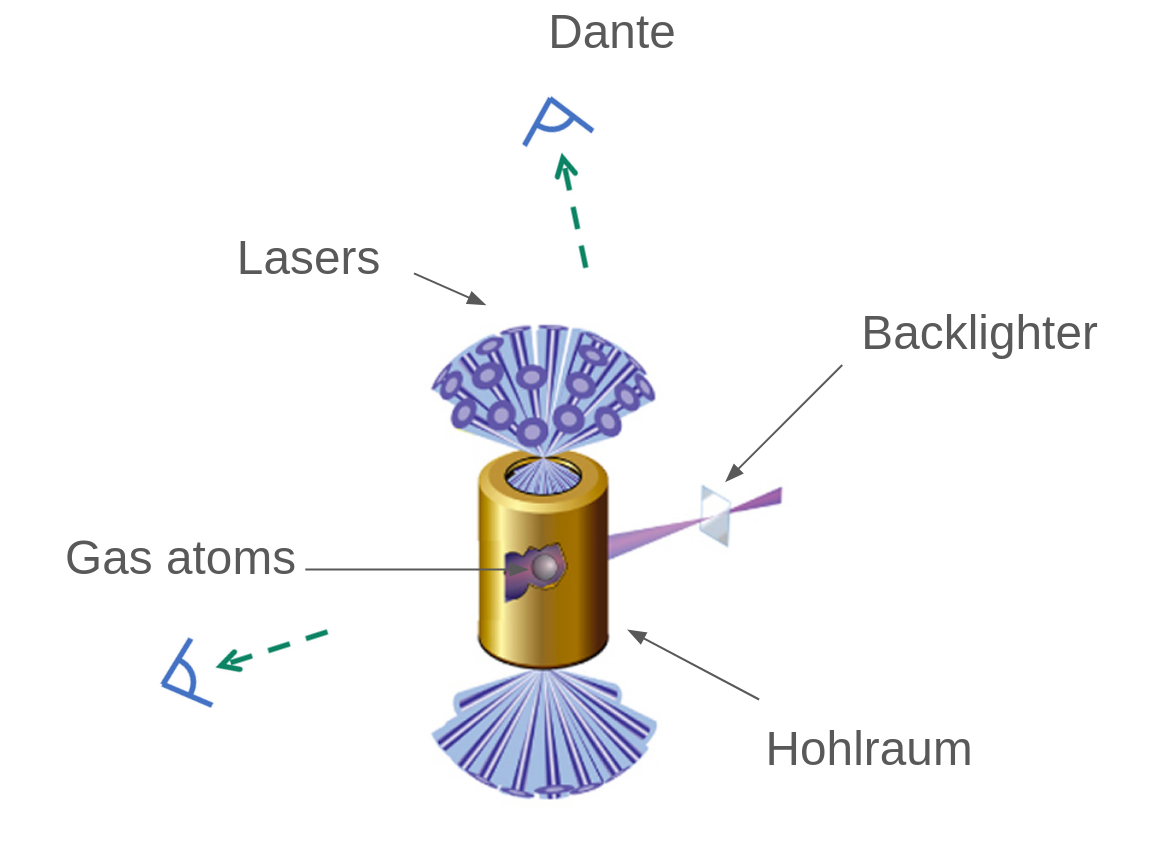
\includegraphics[width=0.5\textwidth]{hohl.png}
    \end{figure}
    
\end{frame}

\begin{frame}{Background Info - Physics}
    \begin{itemize}
        \item Backlighter gives us Bremsstrahlung (Brems)
        \item Hohlraum gives us Blackbody
        \item Goal: Find Blackbody Temp
    \end{itemize}

    \begin{figure}[h]
        \centering
        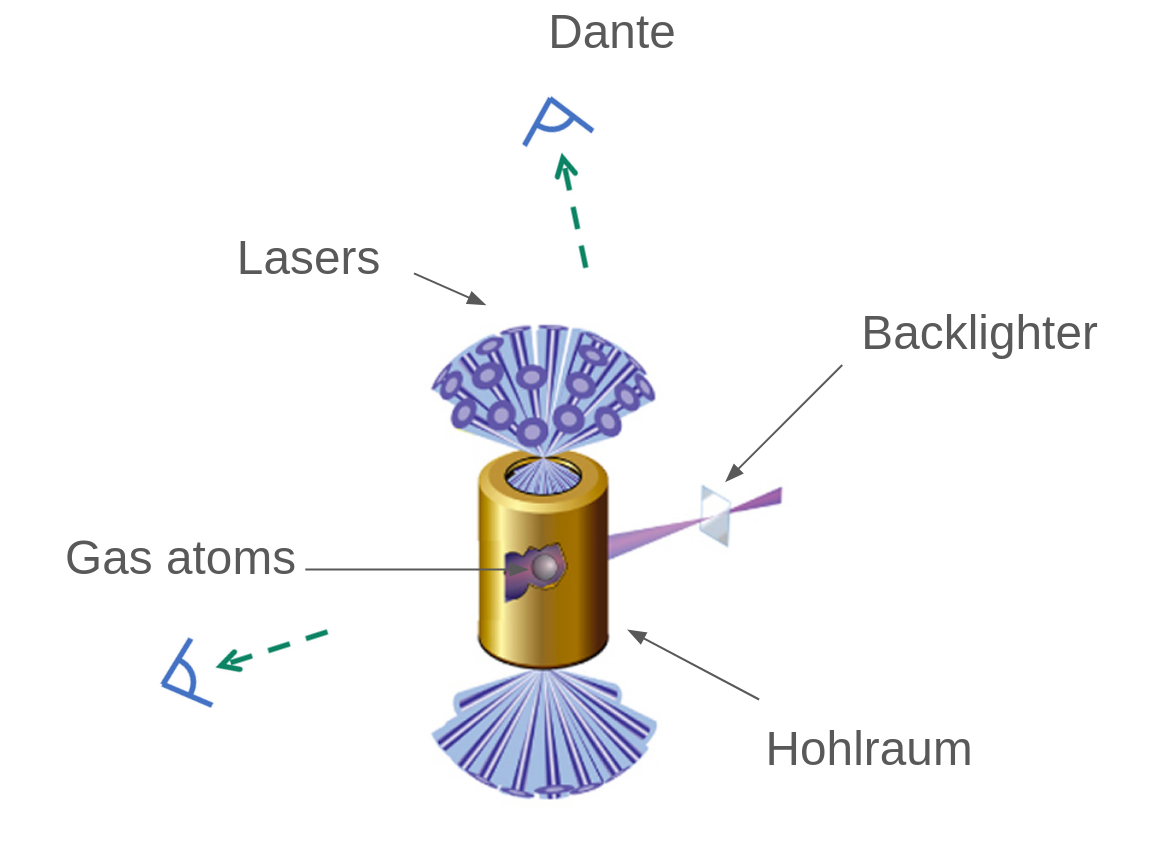
\includegraphics[width=0.5\textwidth]{hohl.png}
    \end{figure}
    
\end{frame}

\begin{frame}{The Problem Is...}

    \begin{itemize}
        \item Signal is MIXED; So how do we disambiguate?
    \end{itemize}
    
    \begin{itemize}
        \item Solution: Use our knowledge of how both behave  
    \end{itemize}


\end{frame}

\begin{frame}{To disambiguate the mixed signal...}

    \begin{itemize}
        \item We have: 
        \begin{itemize}
            \item a curve reading (blackbody + brems)
            \item formulas define how each curve looks like
        \end{itemize}
    \end{itemize}
    \begin{figure}[h]
        \centering
        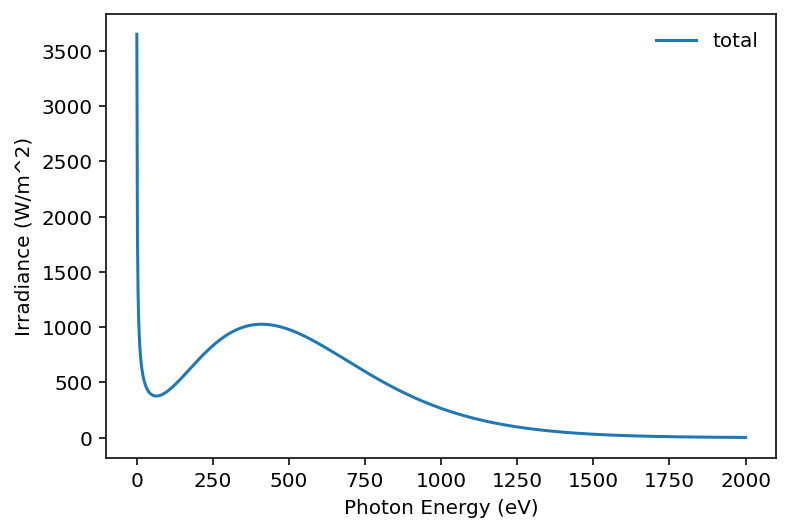
\includegraphics[width=0.5\textwidth]{updatedcurve.png}
    \end{figure}
\end{frame}

\begin{frame}{To disambiguate the mixed signal...}



    \begin{itemize}
        \item The fix: Remodel this curve using formulas
    \end{itemize}
    \begin{figure}[h]
        \centering
        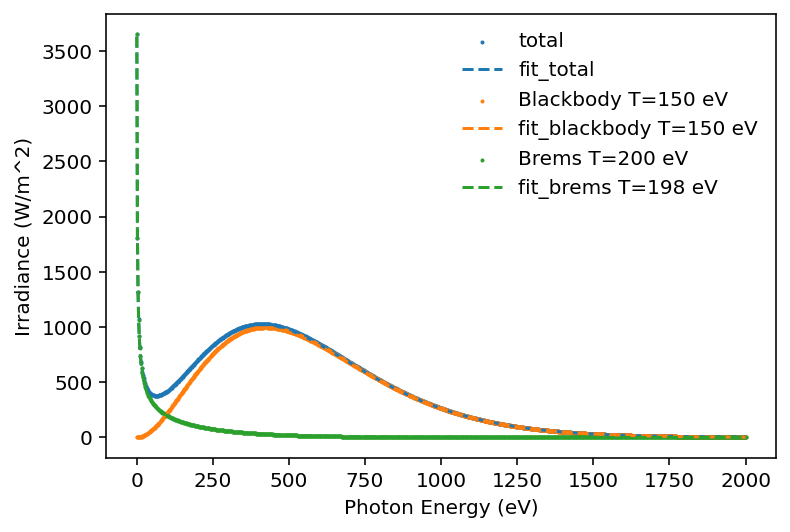
\includegraphics[width=0.5\textwidth]{updatedcurves.png}
    \end{figure}


\end{frame}

\begin{frame}{Formulas!}
    \begin{block}{Blackbody Radiation:}
        \setlength{\jot}{0pt}
        \scriptsize
        \centering
        \begin{align}
            B_\nu(\nu, T) &= \frac{2h\nu^3}{c^2}\frac{1}{\exp\left(\frac{h\nu}{k_B T}\right) - 1} \\
            I_\nu(\nu, T) &= B_\nu(\nu, T)\,\frac{V}{D^2}
        \end{align}
    \end{block}
    \begin{block}{Bremsstrahlung Radiation:}
        \setlength{\jot}{0pt}
        \scriptsize
        \centering
        \begin{align}
            j(\nu, T) &= \frac{8}{3}\sqrt{\frac{2\pi}{3 m_e k_B T}}\,\frac{e_c^6}{m_e c^3}\,Z^2 n_e n_i \, \exp\left(-\frac{E_p}{E_t}\right) \, \bar{g}_{ff} \\[6pt]
            \bar{g}_{ff} &= 1 + 0.1728\left(\frac{E_p}{I_H Z^2}\right)^{1/3}\left(1 + \frac{2E_t}{E_p}\right) \\[6pt]
            I &= \frac{j(\nu,T)\,V}{D^2}  
        \end{align}
    \end{block}
\end{frame}

\begin{frame}{Putting it altogether...}



    \begin{itemize}
        \item Bayesian Models: Metropolis/MCMC and NUTS/HMC
        \item Feed formulas and guesses in models
        \item Find Blackbody Temp
    \end{itemize}


\end{frame}

\begin{frame}{Model Option: Metropolis/MCMC}
    \begin{itemize}
        \item Takes in Blackbody Temp guess 
        \item Uses Formulas to create a 'draw'
        \item Accepts or Rejects draw
    \end{itemize}


\end{frame}
\begin{frame}{Draw #1}
    \begin{itemize}
        \item Model generates 1000s of draws like this: 
    \end{itemize}
    
    \begin{figure}[h]
        \centering
        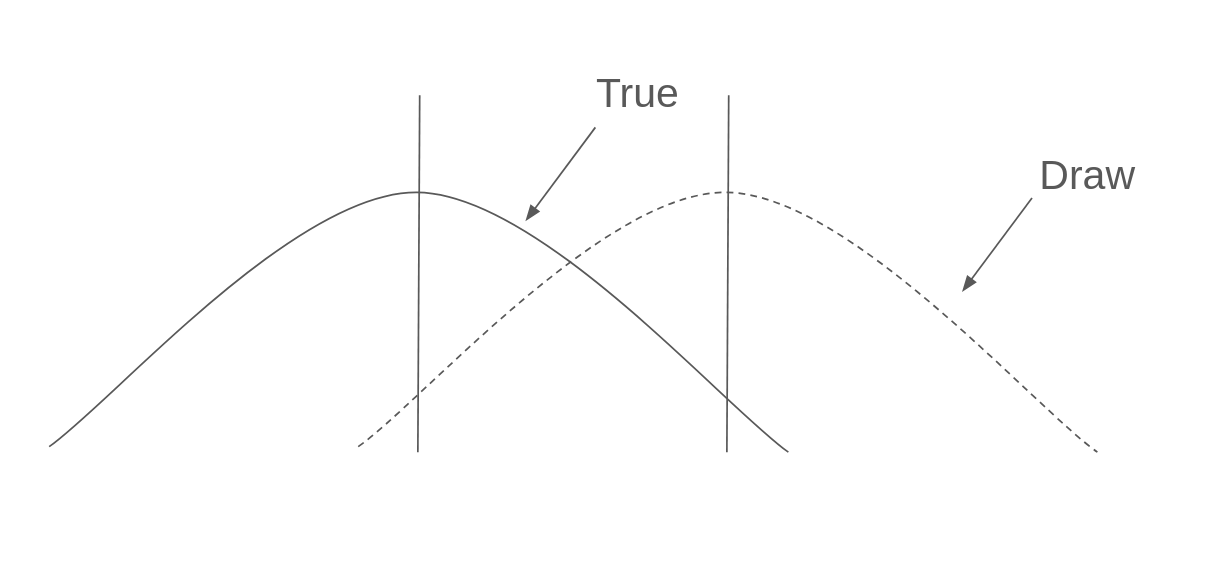
\includegraphics[width=0.5\textwidth]{prop_2.png}
    \end{figure}
    \uncover<2->{Reject} \\
\end{frame}

\begin{frame}{Draw #2}
    \begin{itemize}
        \item Specialty: Learns from previous draw! 
    \end{itemize}
    \begin{figure}[h]
        \centering
        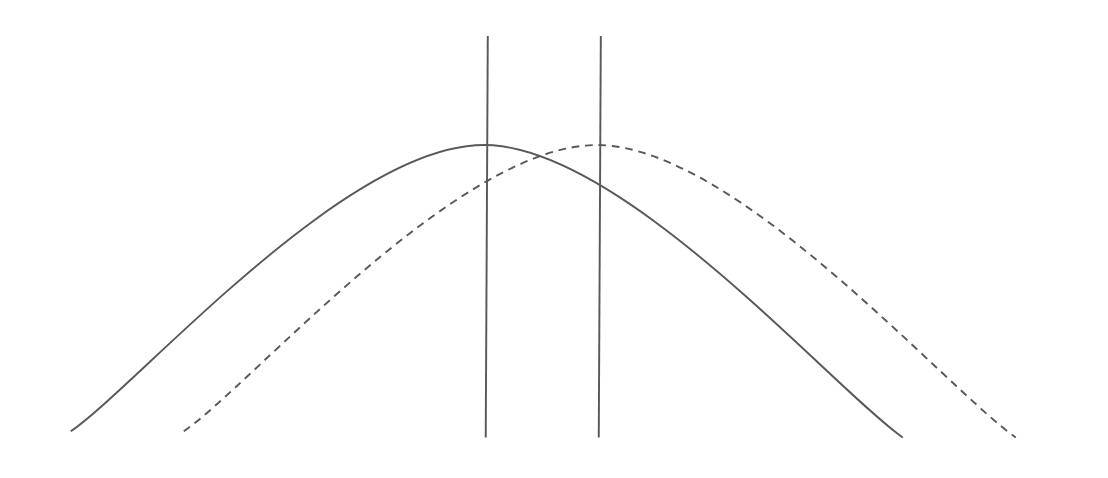
\includegraphics[width=0.5\textwidth]{prop1.png}
    \end{figure}
    \uncover<2->{Accept} \\
    
\end{frame}

\begin{frame}{How all the accepted draws look like...}
    \begin{figure}[h]
        \centering
        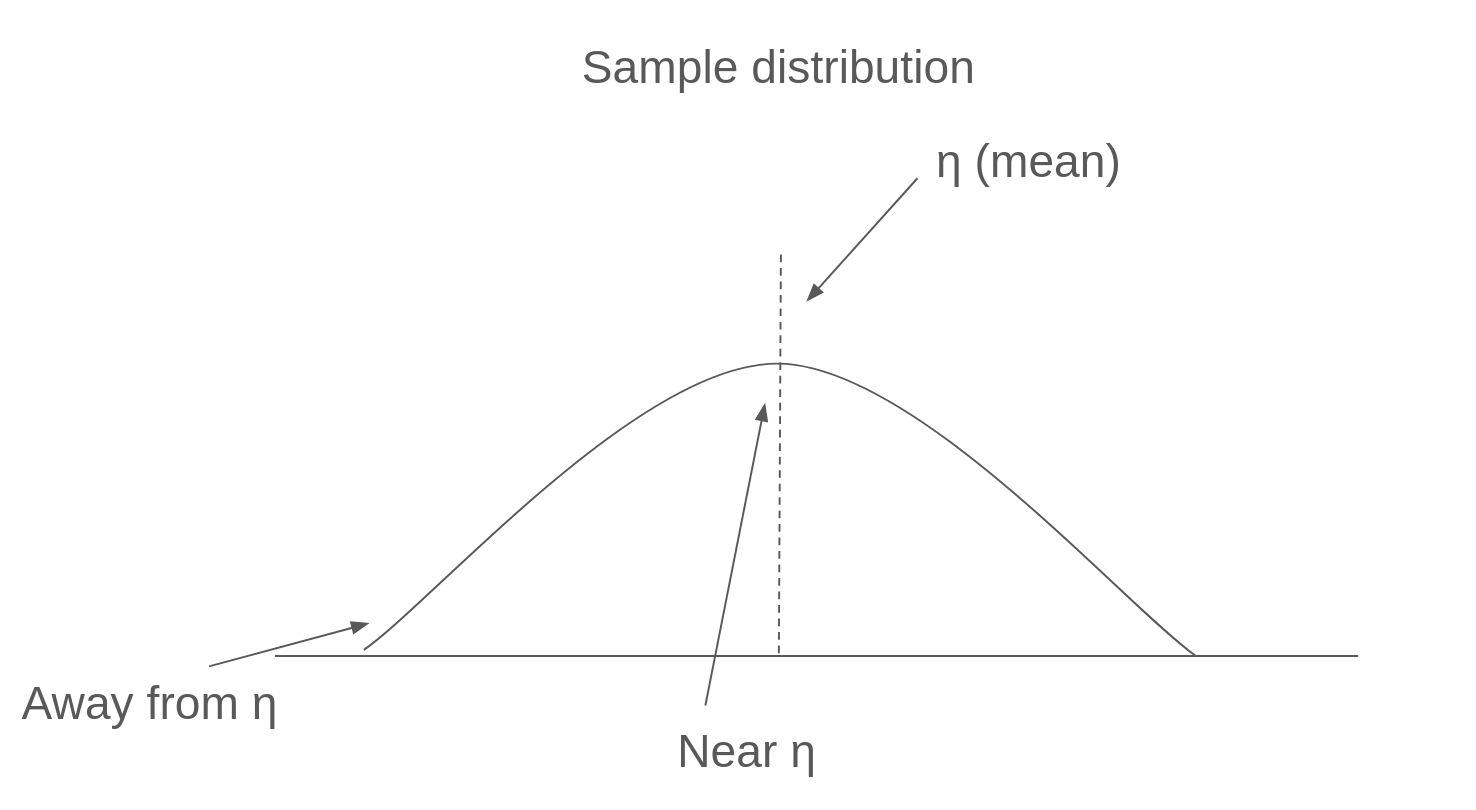
\includegraphics[width=0.5\textwidth]{distribtution.png}
        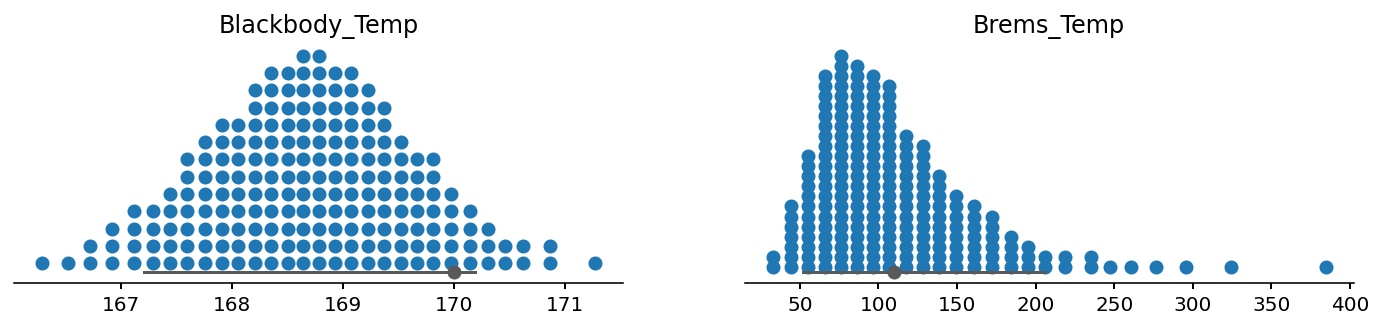
\includegraphics[width=1\textwidth]{posterior-new.png}
    \end{figure}

    
\end{frame}

% \begin{frame}{Methodology - Problem}
%     \begin{itemize}
%         \item Algorithm has Prior (Measured data) 
%         \item We want to find properties from this curve
%         \item We cannot directly find its properties; we don’t exactly know how it's shaped
%     \end{itemize}

%     \begin{figure}[h]
%         \centering
%         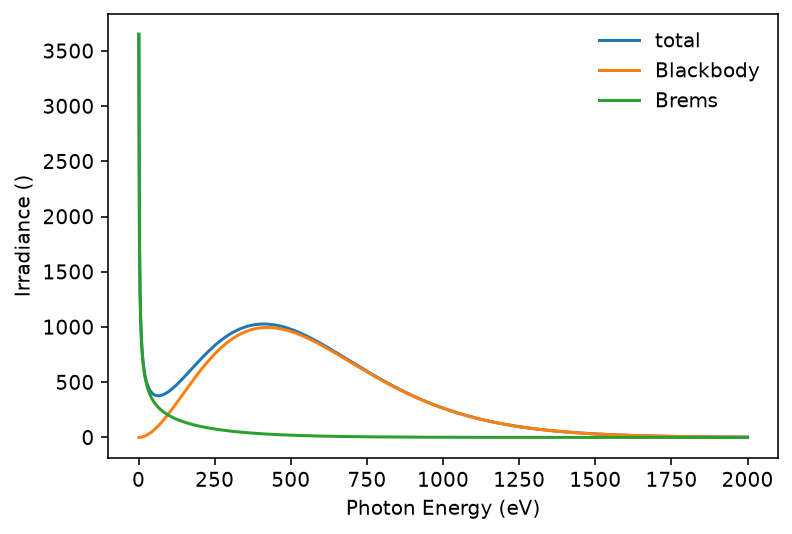
\includegraphics[width=0.5\textwidth]{observed.png}
%     \end{figure}
    
% \end{frame}


% \begin{frame}{Methodology - Solution}
%     \begin{itemize}
%         \item MCMC proposes a curve, generated by formulas 
%         \item MCMC looks at how far this proposed curve is from the actual data
%         \item It keeps or rejects this proposal
%     \end{itemize}
    
% \end{frame}

% \begin{frame}{Formula}
%     \begin{itemize}
%         \item MCMC proposes values for variables 
%         \item Calculates Irradiance for both
%     \end{itemize}

    

%     \begin{block}{Blackbody Radiation:}
%         \setlength{\jot}{0pt}
%         \scriptsize
%         \centering
%         \begin{align}
%             B_\nu(\nu, T) &= \frac{2h\nu^3}{c^2}\frac{1}{\exp\left(\frac{h\nu}{k_B T}\right) - 1} \\
%             I_\nu(\nu, T) &= B_\nu(\nu, T)\,\frac{V}{D^2}
%         \end{align}
%     \end{block}
%     \begin{block}{Bremsstrahlung Radiation:}
%         \setlength{\jot}{0pt}
%         \scriptsize
%         \centering
%         \begin{align}
%             j(\nu, T) &= \frac{8}{3}\sqrt{\frac{2\pi}{3 m_e k_B T}}\,\frac{e_c^6}{m_e c^3}\,Z^2 n_e n_i \, \exp\left(-\frac{E_p}{E_t}\right) \, \bar{g}_{ff} \\[6pt]
%             \bar{g}_{ff} &= 1 + 0.1728\left(\frac{E_p}{I_H Z^2}\right)^{1/3}\left(1 + \frac{2E_t}{E_p}\right) \\[6pt]
%             I &= \frac{j(\nu,T)\,V}{D^2}  
%         \end{align}
%     \end{block}

    
% \end{frame}

% \begin{frame}{Proposal #1}
%     \begin{itemize}
%         \item Irradiances are compared 
%     \end{itemize}
%     \begin{figure}[h]
%         \centering
%         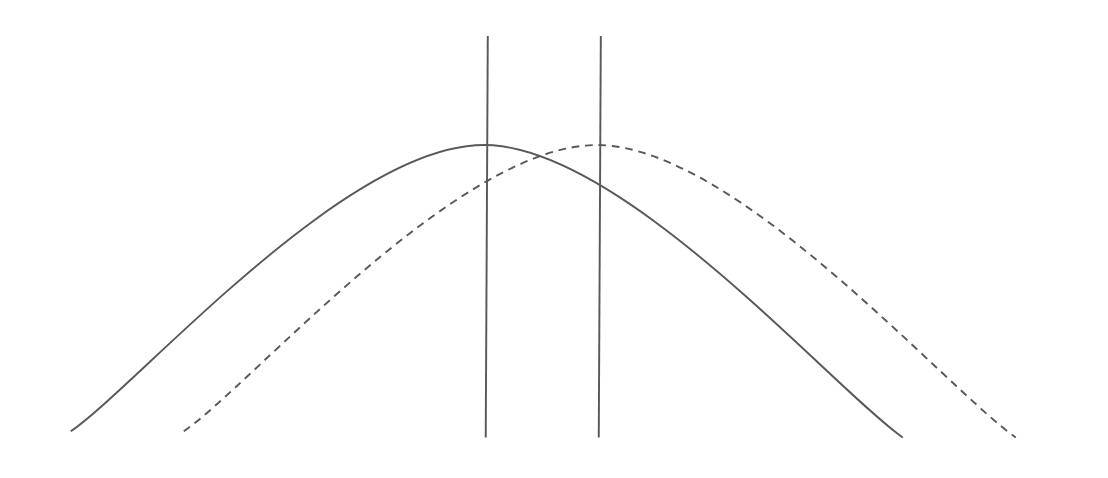
\includegraphics[width=0.5\textwidth]{prop1.png}
%     \end{figure}
%     \uncover<2->{Accept} \\
    
% \end{frame}

% \begin{frame}{Proposal #2}
%     \begin{itemize}
%         \item Irradiances are compared 
%     \end{itemize}
%     \begin{figure}[h]
%         \centering
%         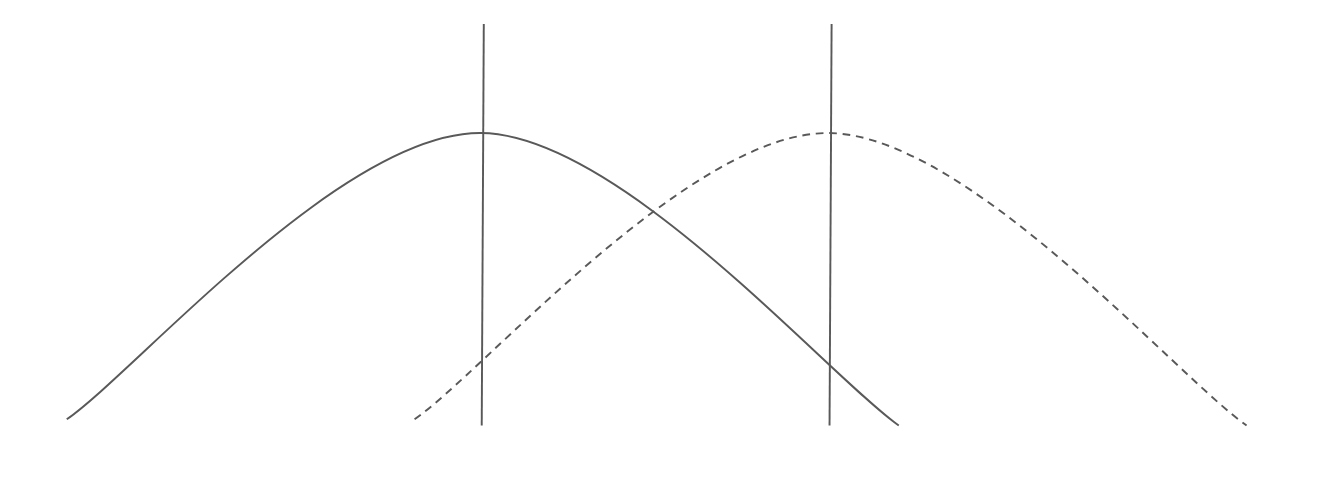
\includegraphics[width=0.5\textwidth]{prop2.png}
%     \end{figure}
%     \uncover<2->{Reject} \\
    
% \end{frame}

% \begin{frame}{How all the accepted draws look like...}
%     \begin{itemize}
%         \item Samples make a distribution
%         \item Mean’s property = True properties
%     \end{itemize}
%         \begin{figure}[h]
%         \centering
%         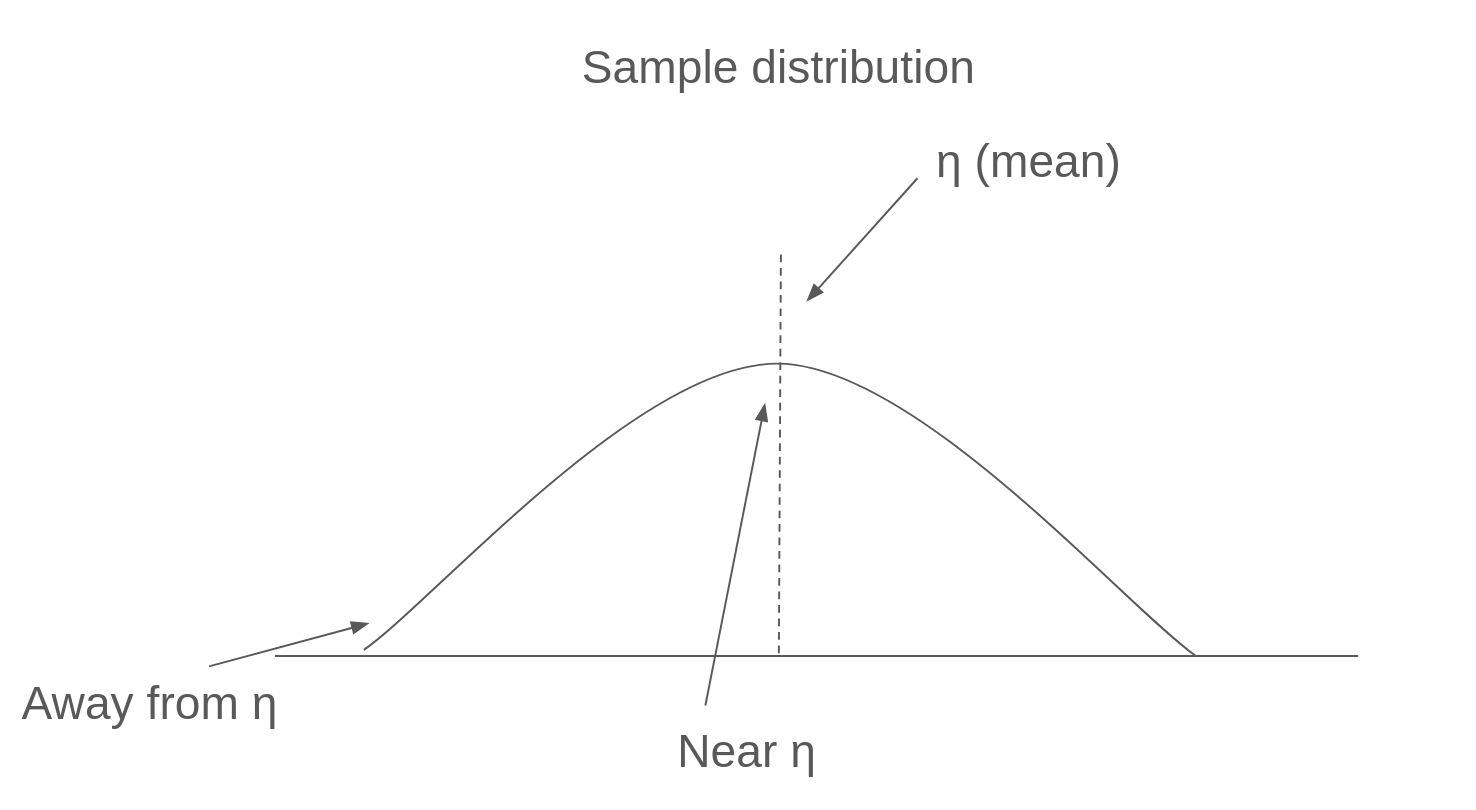
\includegraphics[width=0.5\textwidth]{distribtution.png}
%         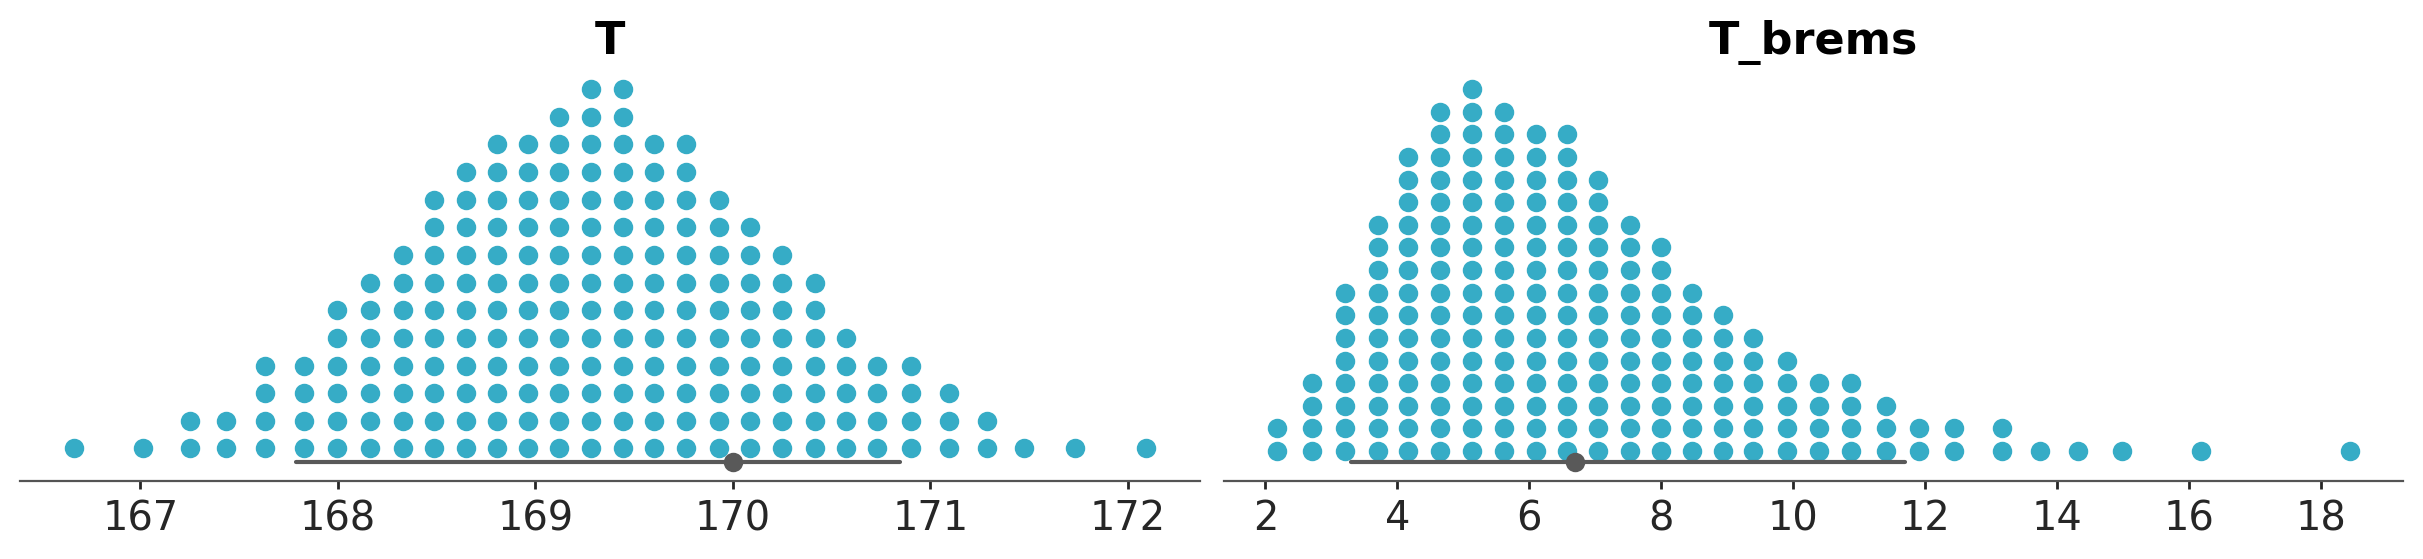
\includegraphics[width=0.5\textwidth]{posterior.png}
%     \end{figure}

    
% \end{frame}
    

\begin{frame}{Model Option: NUTS No U-turn Sampler}
    \begin{itemize}
        \item Lands on the posterior
        \item Picks a direction: Right or Left
        \item Height favored
    \end{itemize}

    \begin{figure}[h]
        \centering
        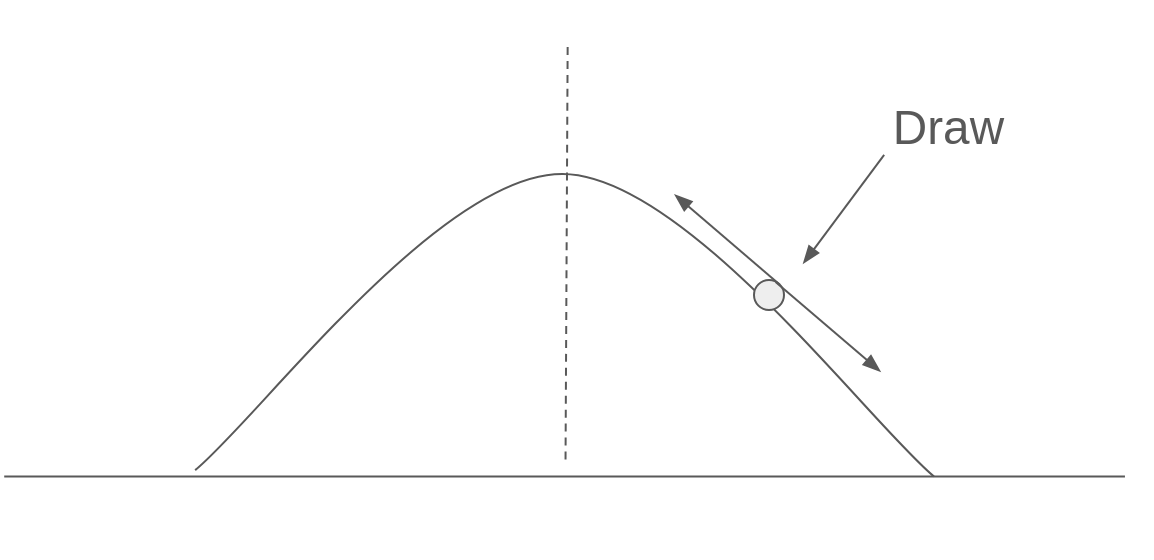
\includegraphics[width=0.75\textwidth]{nuts.png}
    \end{figure}

    
\end{frame}
\begin{frame}{Finding the better model}
    \begin{itemize}
        \item Synthetically created data
    \end{itemize}
        
\end{frame}
\begin{frame}{Fit Comparison}
    \begin{itemize}
        \item Metropolis
        \begin{itemize}
            \item Poor r-hat values
        \end{itemize}
    \end{itemize}
    
    \begin{figure}[h]
        \centering
        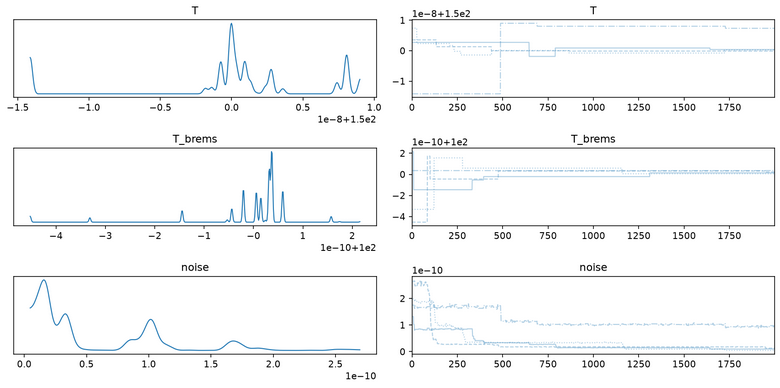
\includegraphics[width=1\textwidth]{metro.png}
    \end{figure}
    
\end{frame}

\begin{frame}{Fit Comparison}
    \begin{itemize}
        \item Hamiltonian (No-U-Turn or NUTS)
        \begin{itemize}
            \item Good r-hat values
        \end{itemize}
    \end{itemize}
    
    \begin{figure}[h]
        \centering
        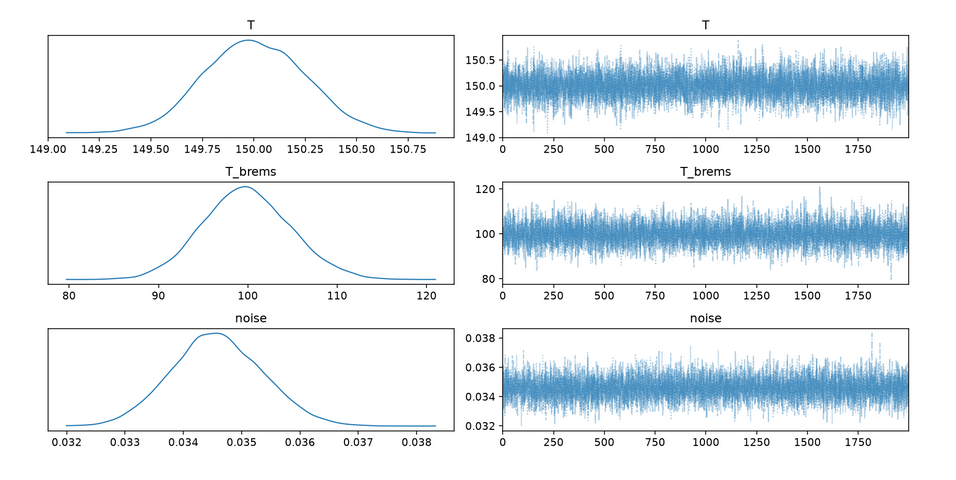
\includegraphics[width=1\textwidth]{hmc.png}
    \end{figure}
    
\end{frame}

\begin{frame}{Result}
    \begin{itemize}
        \item NUTS Model proved to be superior
        \item Next step: performance with noise
    \end{itemize}
        
\end{frame}

\begin{frame}{Introducing Noise to NUTS}
    \begin{itemize}
        \item MSE: Difference between measured and fit
        \begin{itemize}
            \item Low MSE = good fit
            \item High MSE = poor fit
        \end{itemize}
    \end{itemize}
    
    \begin{figure}[h]
        \centering
        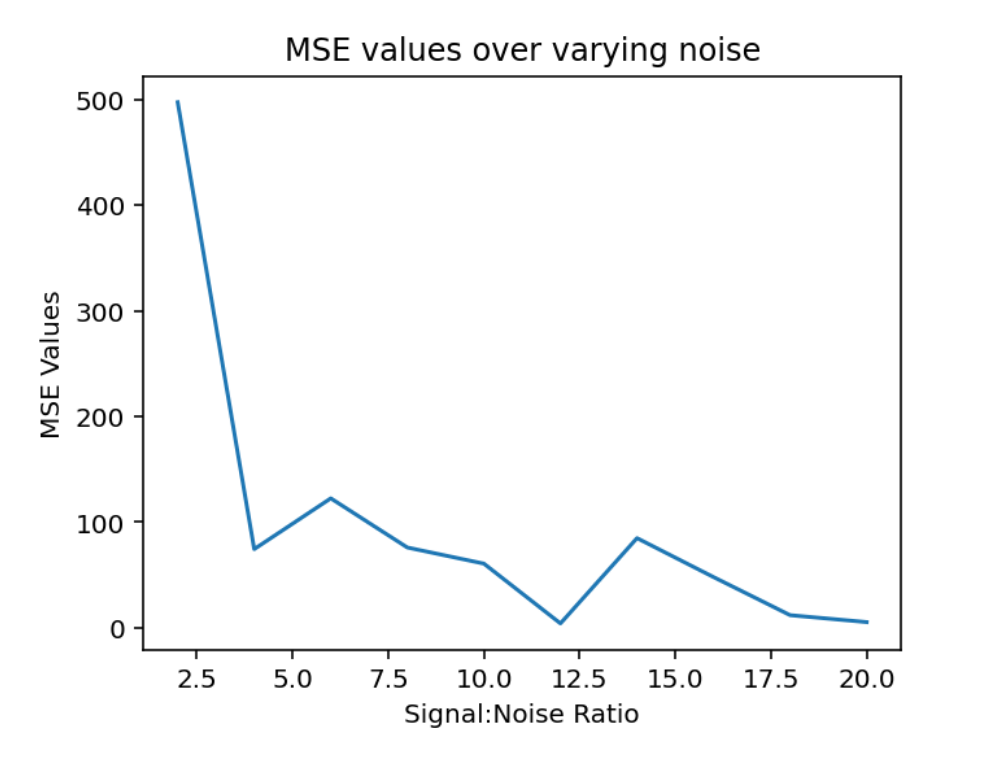
\includegraphics[width=0.5\textwidth]{newmse.png}
    \end{figure}
    
\end{frame}


\begin{frame}{Introducing Experimental Data to NUTS}
    \begin{itemize}
        \item Purpose: see irradiance evolve
        \item Choppy
        \item Random spike 
    \end{itemize}
    
    \begin{figure}[h]
        \centering
        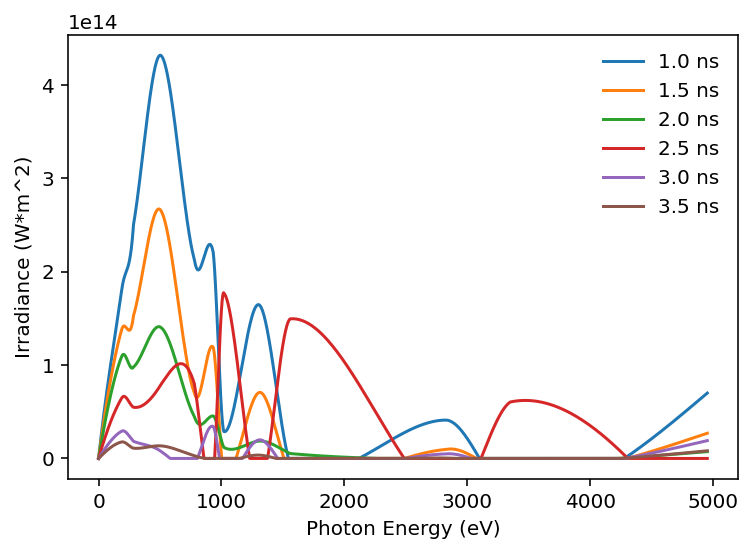
\includegraphics[width=0.5\textwidth]{fit_dante.png}
    \end{figure}
    
\end{frame}


\begin{frame}{Introducing Experimental Data}
    
    \begin{figure}[h]
        \centering
        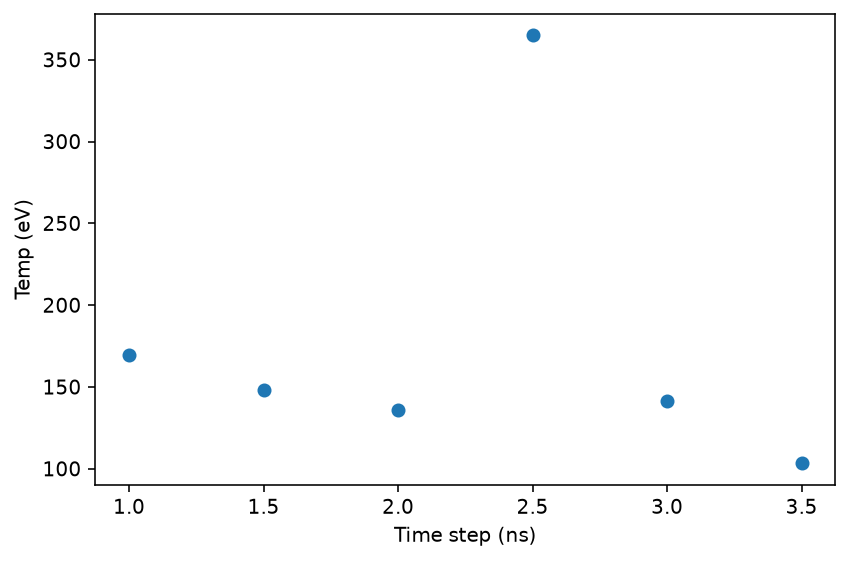
\includegraphics[width=0.5\textwidth]{compare-temp-time.png}
        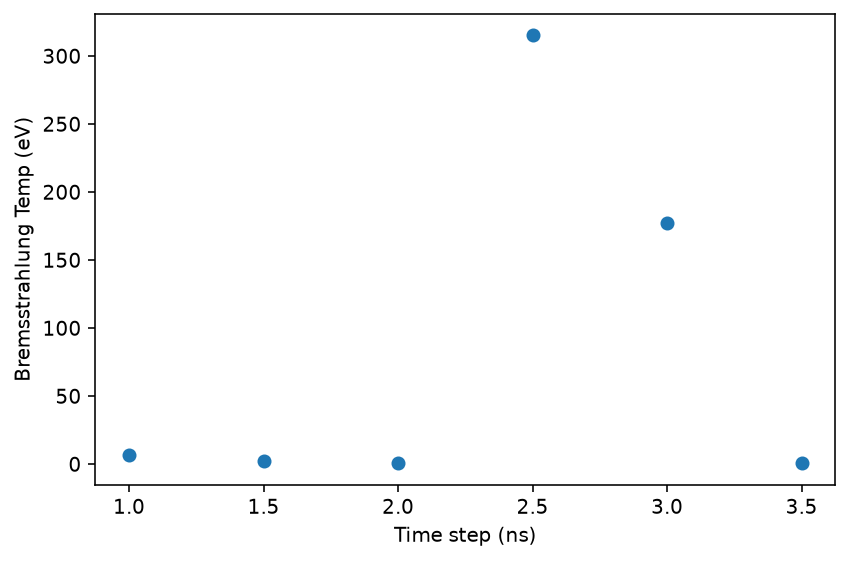
\includegraphics[width=0.5\textwidth]{compare-brtemp-time.png}
    \end{figure}
    
\end{frame}

\begin{frame}{Some changes had to be made...}
    \begin{itemize}
        \item Adding an Amplitude term
        \item Normalizing data 
        \item Failed to bump up Brems
    \end{itemize}

    \begin{figure}[h]
        \centering
        
\includegraphics[width=0.5\textwidth]{fit_of_all_curves.png}
    \end{figure}
    
\end{frame}





\begin{frame} {Advancements}
    \begin{itemize}
        \item Address backlighter implosion spike  
        \item Account for the M-band gold emission
        \item Explore more Bayesian models
    \end{itemize}

\end{frame}


\begin{frame}{Conclusion}
    \begin{itemize}
        \item Experimental Data: 
            \begin{itemize}
                \item Blackbody T: around 170 [eV]
                \item Brems T: around 7 [eV] * Failed
            \end{itemize}

        \item  Using Metropolis MCMC and NUTS HMC
        \item  NUTS worked well with noise
            \begin{itemize}
                \item Appropriately distorted with noise
                \itme Good fit metric values
            \end{itemize}
        \item  Improvements on toy model
    \end{itemize}

\end{frame}

\begin{frame} {Sources}
    \begin{itemize}
        \item https://lasers.llnl.gov/for-users/experimental-capabilities/capsule-implosions
        \item https://www.sciencedirect.com/journal/high-energy-density-physics
    \end{itemize}
    
    
\end{frame}


\begin{frame}
    \centering
    Questions? 

\end{frame}


\end{document}